\section{Analyzing ESBL E. coli solates from patients of the University hospital Basel}
Our collaborator, head of the clinical microbiology from the University hospital Basel, collected 65 isolates of 34 patients who had inlfammations caused by ESBL E. coli. Over all the sampling period was approximately four and a half years. Sample collection for one patient typically happened within several months. \\
His group determined the MIC of the extended cephalosporines cefepime and ceftazidime for every collected isolate  and short-read sequenced them on a MiSeq Illumina system. Only samples were included where ESBL genes were detected. This resulted in a collection with multiple isolates per patient, where a change of MIC for cefepime and ceftazidime was visibile over time caused by gained or lost resistance.\\
Only a few patients showed a significant change in the MIC of cefepime or cefatzidime over time so only those patients of interest could be included in the analysis.  

\subsubsection{Illumina sequencing}
Illumina sequencing was done by our collaborators from the clinical microbiology from the University hospital of Basel. They extracted the DNA from cultured samples using the EZ1 DNA tissue kit on an EZ1 Advanced XL robotic system (Qiagen). The library for the sequencing was prepared using the Nextera XT library preparatino kit (Illumina). The resulting library was sequenced using a MiSeq Illumina platform \cite{nanopore}. The reads produced with Illumina were trimmed with Trim Galore \cite{noauthor_babraham_nodate}.

\subsubsection{Nanopore sequencing}
Isolates from patients of interest were sequenced with a MinION from Oxford Nanopore. Each library was prepared with a ligation sequencing kit (LSK-108) followed with the native barcoding expansion kit allowing barcoding every sample and loading all of them on a single flow cell (FLO-MIN106D). A detailed protocol of the library preparation is available in the publication of Noll et al \cite{noauthor_resolving_nodate}.

\subsection{Phylogenetic analysis}
Before the genomes of the isolates coming from one patient could be compared phylogenetic analyis had to be done.
This was necessary in order to ensure, that one patient was infected with the same ESBL E. coli strain over the whole sampling period. This was done by using the panX tool.\\
PanX is a tool which allows to build a phylogenetic tree, which contains the information about how closely related strain are. It's a tool which clusters genes into orthologous groups. From these clusters, panX identifes the core genome which are genes shared by all strains in a group of isolates \cite{ding_panx:_2018}. Based on those core genomes a strain-level phylogeny can be build, making use of single nucleotide polymorph positions (SNPs). \\ 
The output of panX is a tree, which visualizes how closely related different isolates are. If isolates have the same common ancestor they map on the same clade of the tree. Based on the SNPs in the core-genome  the strains are further distinguished and map on different branches
PanX takes annotated genomes as input files, that's why every sample was short-read assembled and annotated.

\subsubsection{Short read assembly and genome annotation}
Since every isolate was short-read sequenced, all of them were included for the phylogenetic analysis. For assembling spades (v3.12.0) \cite{nurk_assembling_2013} was used. The output of spades was a short-read assembly containing about 100 contigs per assembly. For E. coly only a handful of contigs are expected which shows how important long-reads are in order to get structural accurate whole-genome assemblies. But using just short reads was enough because the assembly was only used to identify all genes of every isolate.
Identification of the genes was done with prokka (v.1.12) \cite{seemann_prokka:_2014}. Prokka first searches a core set of well chacracterized protein using BLAST+ and then compares reading frames to a database derived from UniProtKB \cite{seemann_:zap:_2019}. The results from prokka were stored in a genbank file for every isolate. Based on those genbank files, the phylogenetic tree was built with panX. 
\label{section:annotation}

\subsection{Identification of SNPs}
\begin{figure}
	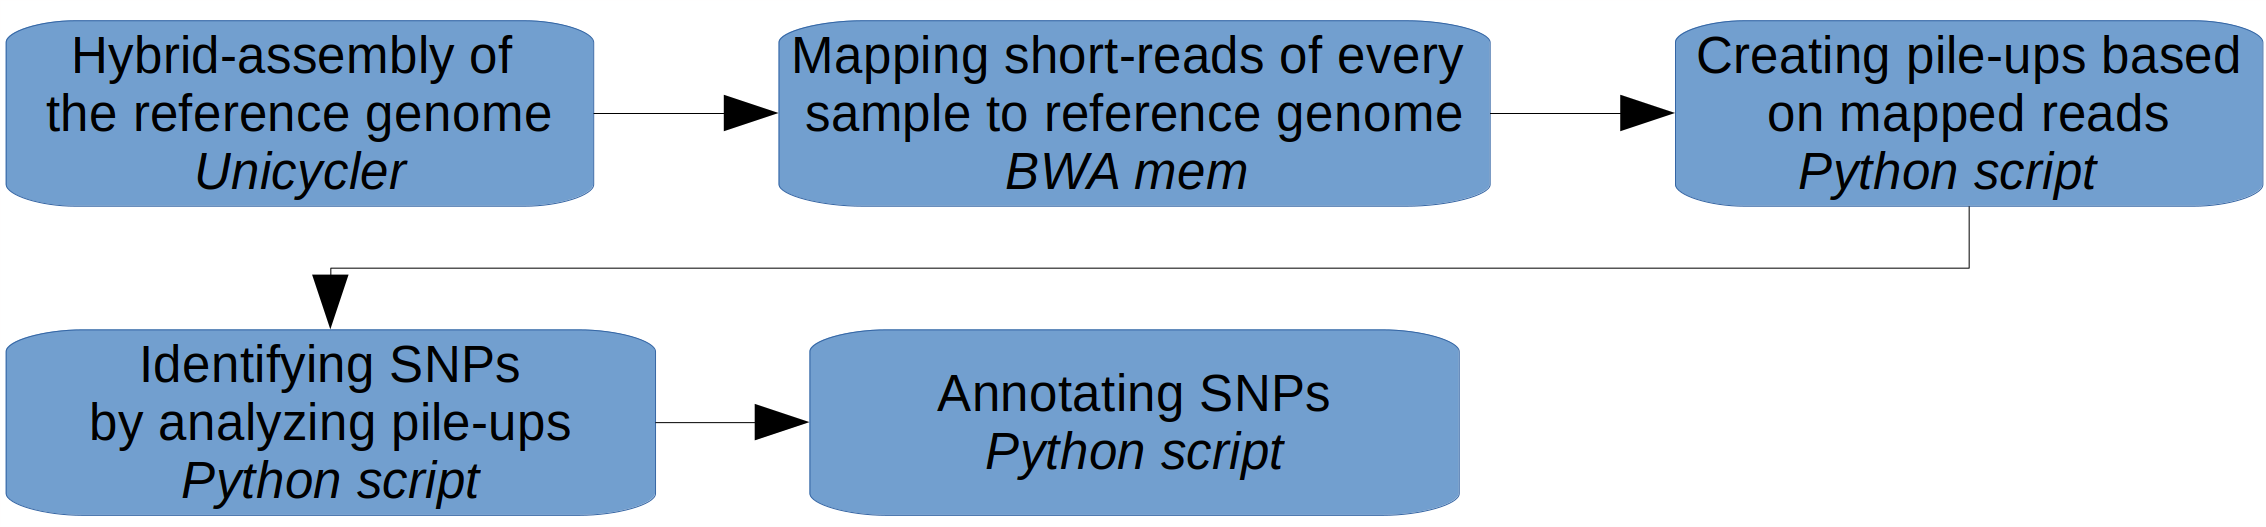
\includegraphics[scale=0.2]{pipeline.png}
	\caption{Pipe line used for the identification of SNPs and affected genes and promotors}
	\label{figure:pipeline}
\end{figure}
For identifying mutations in form of SNPs a bioinformatical pipeline with five steps was established as shown in Figure \ref{figure:pipeline}. Using this pipe line it was possible to identify SNPs which accumulated over time. 

\subsubsection{Creating a reference genome}
As a first step of the pipeline a reference genome was built for every patient of interest. This was done by combining the Illumina and Nanopore sequencing data of the isolate with the lowest MIC of cefepime and ceftazidime from each patient of interest into a hybrid assembly using Unicycler \cite{wick_unicycler:_2017}. \\
Annotation of every build reference genome was done by identification of all genes using prokka \cite{seemann_prokka:_2014} (see section \ref{section:annotation}). Additionally promotor regions were identifed 
using the promoter prediction tool PePPER \cite{pepper} and the promoter data base hosed on EcoCyc \cite{ecocyc}. PePPER is a tool which takes the assembled sequence as an input and predicts promotor sequences which are returned. Those sequences were mapped against the reference genome using graphmap \cite{sovic_fast_2016}. Furhtermore a promotor data base hosted on EcoCyc was used which contains around 3800 experimentally validated promotors. The sequences from this database was downloaded and every sequence mapped against the reference genome with graphmap. Mapping of PePPER and from the EcoCyc data base was stored in a seperate bam-file for every reference genome. 
\label{section:annotatiion_ref}
\subsubsection{Mapping of short reads}
As a next step all the Illumina short-reads from every isolate of each patient of interest were mapped against the reference genome with BEW mem \cite{li_fast_2009}. This resulted in a bam file for every selected sample

\subsubsection{Creating pile ups}
For identifying SNPs pile ups are used. Pile ups are count matrices which store how many times which nucleotide is present at a certain position in the genome. Based on those count matrices coverage or base frequency can be calculated, or by comparing pile ups from different isolates of the same patient, it's possible to identify SNPs. Identifying SNPs this way was only possible, because all the short-reads were mapped against the same reference genome.\\
The pile ups were created for every sample of the selected patients with a custom \href{https://github.com/nahanoo/ESBL\_project/pileup.py}{pileup.py} script. The script iterated over every position in the reference genome. Then it checked which base was present in every read which was mapped to this position and stored the nucleotide counts in a matrix. All the pile ups from one patient were stored in a matrix stack. This allowed to easily compare the most abundant base, coverage or base frequency at a certain position over every sample of a patient.

\subsubsection{Identification of SNPs} 
For identification of SNPs a python script \href{https://github.com/nahanoo/ESBL\_project/pileup.py}{analysis\_modular.py} was used. This script went though every position in the reference genome. Using the pile ups it was then checked which base was the most abundant compared to the according position of the reference genome. . This means if a different base was abundant in a pile up than in the reference genome, a SNP was identified. All the SNPs were stored in a new matrix. Filtering to every found SNP was applied by checking the coverage and base frequency of every SNP in the pile ups. Only SNPs where the coverage was at least 30 and the base frequency was at least 0.8 were kept for further analysis. 

\subsubsection{Identification of genes and promotors affected by SNPs}
As a last step as seen in Figure \ref{figure:pipeline} it was checked if annotation was available for every found SNP. As described in section \ref{section:annotatiion_ref} genes and promotors were identified for every reference genome. \\
For checking if a SNP affected a gene, we analyzed the genbank file with \cite{cock_biopython:_2009}. We checked if a SNP was located between a start and an end position of a gene which was stored in  the genbank file, where also the information about the gene and the product was available. For checking if a SNP affected a promotor region, we went through the bam-file created based on PePPER and EcoCyc (see \ref{section:annotatiion_ref}). We checked if a SNP is loacted between a start or end positon of a mapped promotor sequence. 


%%%%%%%%%%%%%%%%%%%%%%%%%%%%%%%%%%%%%%%%%%%%%%%%%%%%%%%%%%%%%%%%%%%%%%%%%%%%%%%%%%%%%%%%%%%%%%%%%%%%%%%%%%%%%%%%%%%%%%%%%%%%%%



\section{Assembling and handling procedure of the morbidostat}
Initially the first morbidostat was build by Toprak et al. \cite{morb_toprak}. The following system is an adapted version of Topraks built differing mainly in it's pump system, controlling unit and software. Hardware which was not commercially available was built by the in-house mechanic and electronic workshop.

\subsection{Hardware and setup}

\begin{figure}[H]
	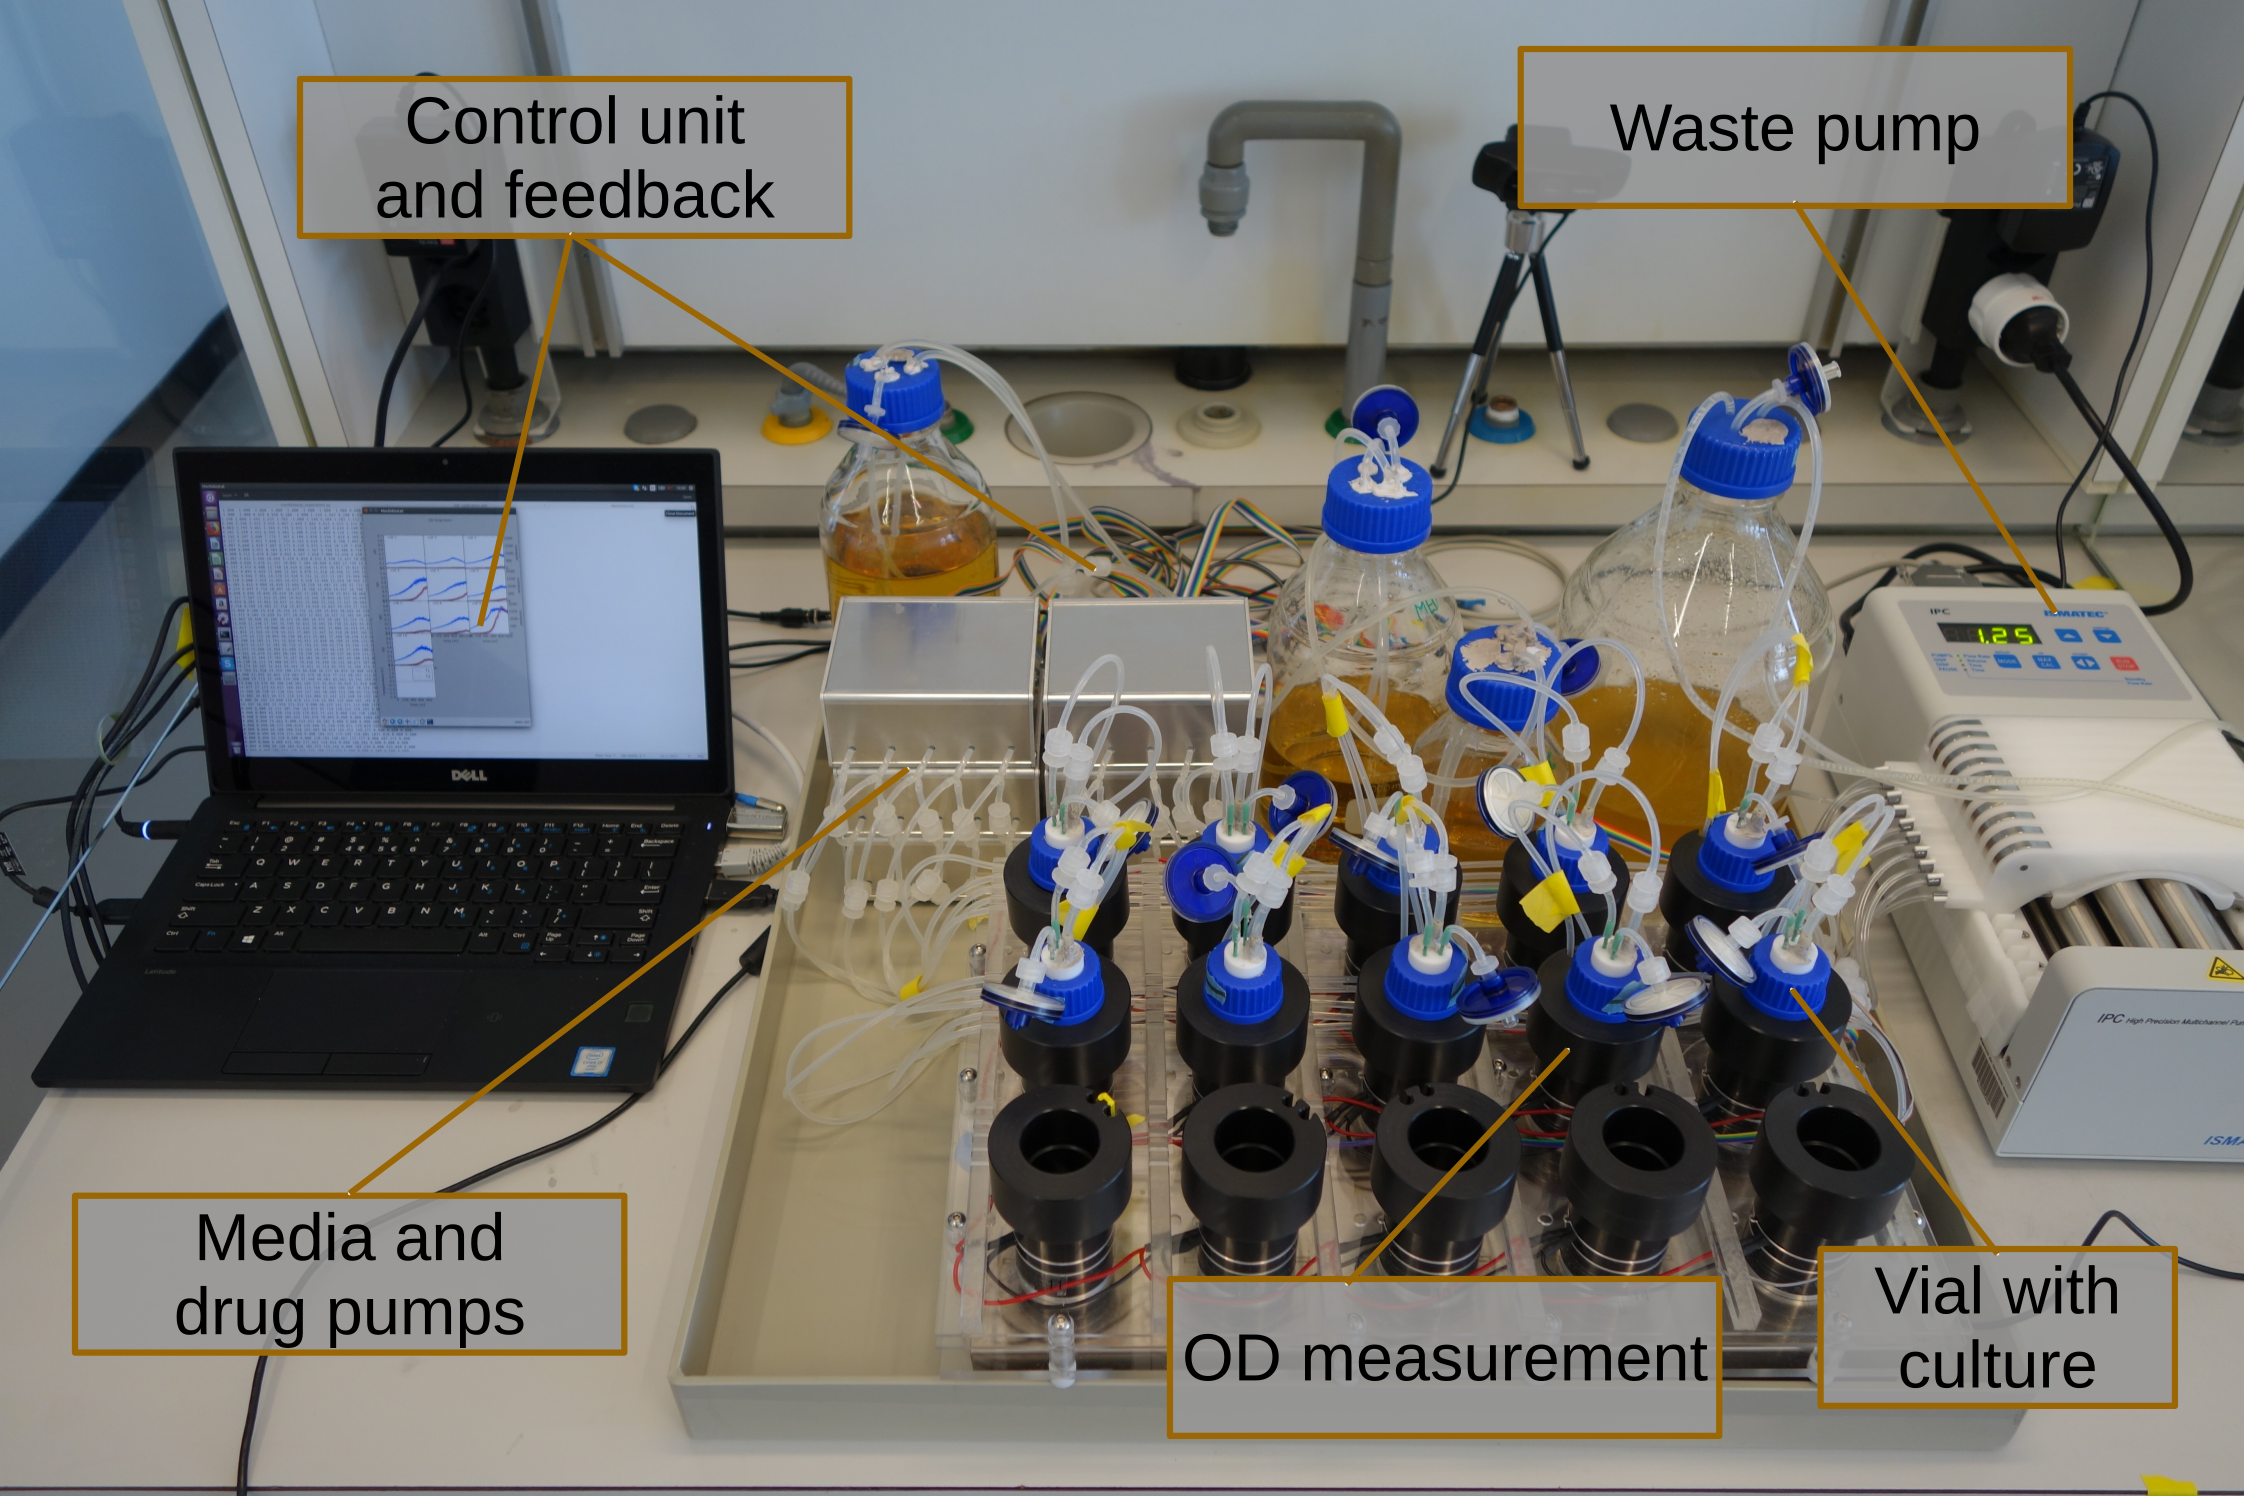
\includegraphics[scale=0.7]{setup_annotated_inksacpe.png}
	\caption{Overview of the morbidostat setup. The arduino (controller) is located behind the drug and media pumps.}
	\label{figure:morbidostat_setup}
\end{figure}  
Figure \ref{figure:morbidostat_setup} shows the morbidostat setup.
The whole setup was placed on a magnetic stirrer which can hold 15 vials. The magnetic stirrer was responsible for a constant mixing of the cultures. On the magnetic stirrer vial holders were placed (black rings visible in Figure \ref{figure:morbidostat_setup}). In those vial holders the OD measuring unit was integrated. It consisted of an LED and a detector which measured scattered light. The cables leading to the vial holders and  connecting the electronics for measuring the OD are visible in Figure \ref{figure:morbidostat_setup}. What can not be seen is that those cables are connected to an arduino which was located behind the pumps. Every vial was connected to four pumps. Three pumps were capable to inject two differenct drug concentrations and media, the fourth pump was used in order to remove volume which exceeded the culture volume (waste). The connections to the pumps and the bottles were made using silicon tubing and plastic luers. \\
For controlling the hardware  the arduino was used, who processed the OD measurements and turned on/off the pumps which led to fluid injection or waste removal.
In Figure \ref{figure:morbidostat_setup} the morbidostat was built up in the open, for later experiments the morbidostat was placed in an hypoxi-station within a biosafety level 2 lab. This was necessary in order for temperature regulation but also for safety reasons (also see section PLACEHOLDER).  

\subsubsection{OD measurements}
For measuring the OD a combination of a light emitting diode (LED) and a phototransistor was chosen. The principle is, that cells cause scattering of a ray of light. By placing an LED at the glass wall of the vial and a phototransistor as a detector in a 135 \degree \space angle, the scattering of the light could be measured. More cells caused more scaterring which caused more light reaching phototransistor because its angled orientation. \\
As a LED OPB608A was chosen from TT electronics with a peak wavelength of 890 nm. For detection a PT 333-3C phototransistor was used. One OD measurement is made possible by two independent circuits which are both connected to a 5 V power source and a ground. As shown in figure \ref{figure:OD_cirguit} one circuit (colored orange) was powering the LED with a x \textOmega resistor connected in serial after the LED. The other circuit (colored blue) was responsible for measuring the scattering of the light with the phototransisitor. 15 OD measuring units were split up in three parallel-conncected chains representing one row of 5 vials. \\
Measuring the scattering worked as follows: Light reaching the phototransistor caused an opening in the semiconductor from the phototransistor which led to a current reaching the tranisistor. The tranistor amplified the current. As visible in the blue colored circuit in Figure \ref{figure:OD_cirguit} a resistor was connected in serial after the phototranisistor. Over this resistor the voltage difference was mesured with the arduino. The opening of the semiconductor was proportional to the light which reached it. A bigger opening led to more current which got amplified even more by the tranisistor. If more current was reaching the resistor over which the voltage was measured, this led to a smaller voltage. In order to get an actual OD, calibration was needed. The voltages were measured which were generated by placing vials with a cell suspension with a certain OD. Because of the linear correlation between the flowing current and the light reaching the phototransistor the correlation between detected voltage and OD could be described in a linear equation.  
In order that sensitivity of the OD measurement could be changed a potentiometer was added in serial before the voltage measurement with the arduino. It turned out that the system was not as sensitive as thought in advance, so all the potentiometers were opened as much as possible meaning that the highest possible resistor was chosen.   

\begin{figure}
	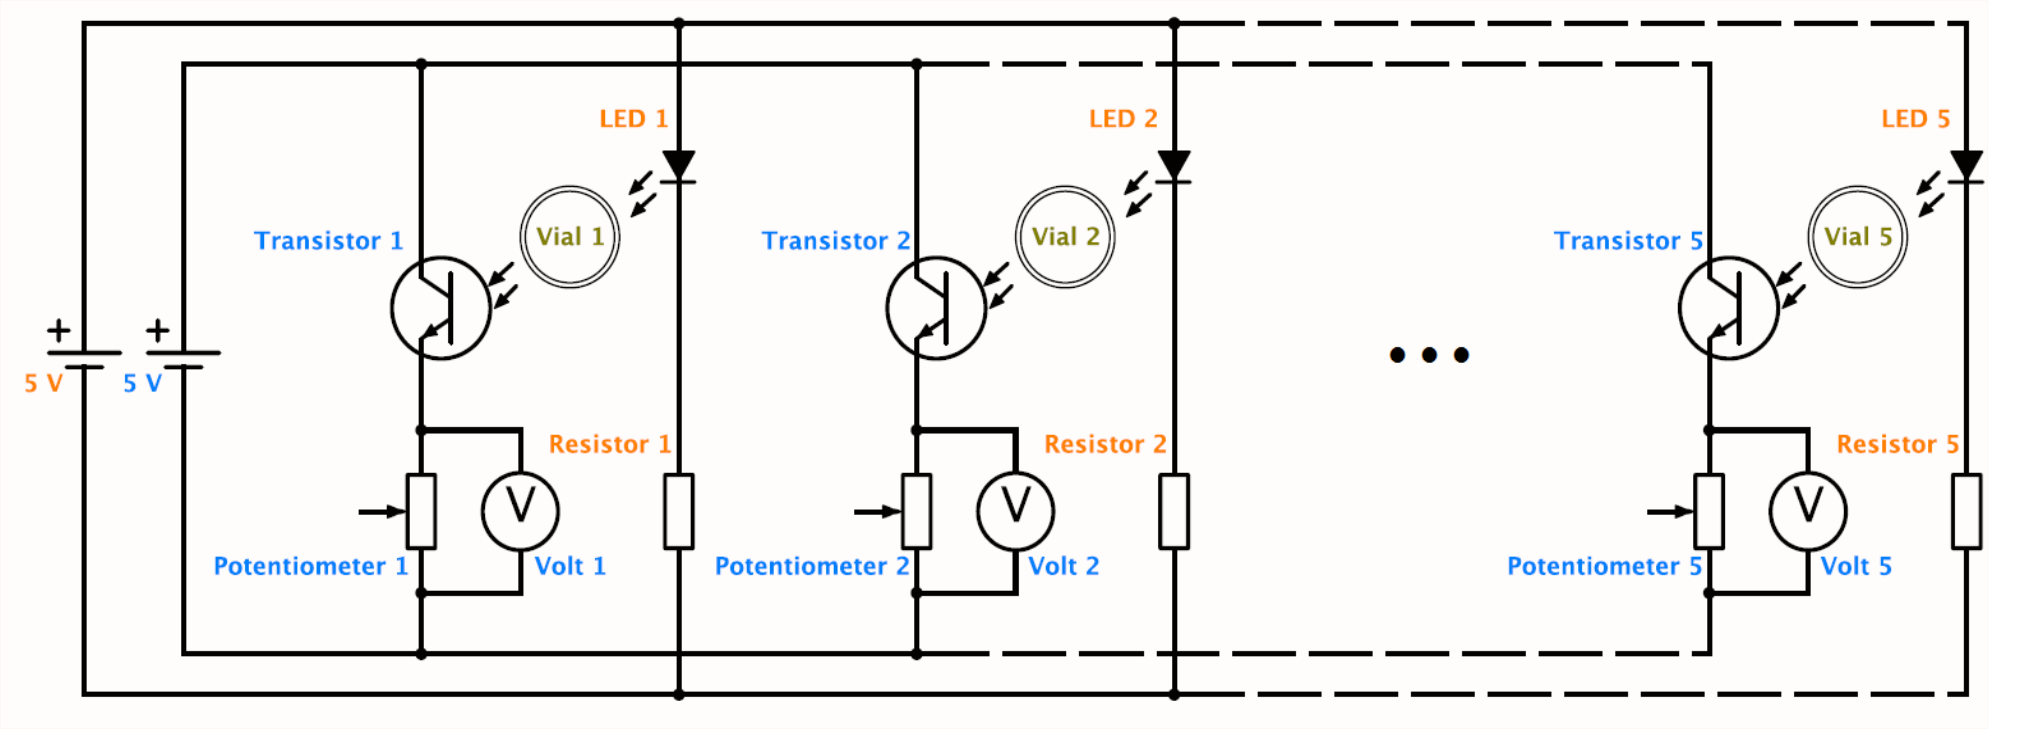
\includegraphics[scale=0.15]{OD_setup.png}
	\caption{Circuit diagram of parallel-connected LED (orange) and phototransistors (blue). This circuit is done independently three times for five vials each. The detector and the LED are orientated in a 135 \degree  angle since this is the best angle for light detection.}
	\label{figure:OD_cirguit}
\end{figure}

\subsubsection{Vials and tubing}
Every vial was connected to three injecting pumps and one pump which removed the waste. This would have led to four tubes connected to a vial. In order to make the vials more accessible we connected the three tubes from the media and drug pumps together and led the connected tube to the vial which is visible in the right Figure \ref{figure:vial_setup}. Two more inlets per vials were necessary which is also shown in the left figure in \ref{figure:vial_setup}. One inlet set to the height of the desired culture volume was used to connect the waste pump. The last inlet was connected to an air filter which was necessary to equalize the pressure within the vial. 

\subsubsection{Pumps} 
\begin{figure}
	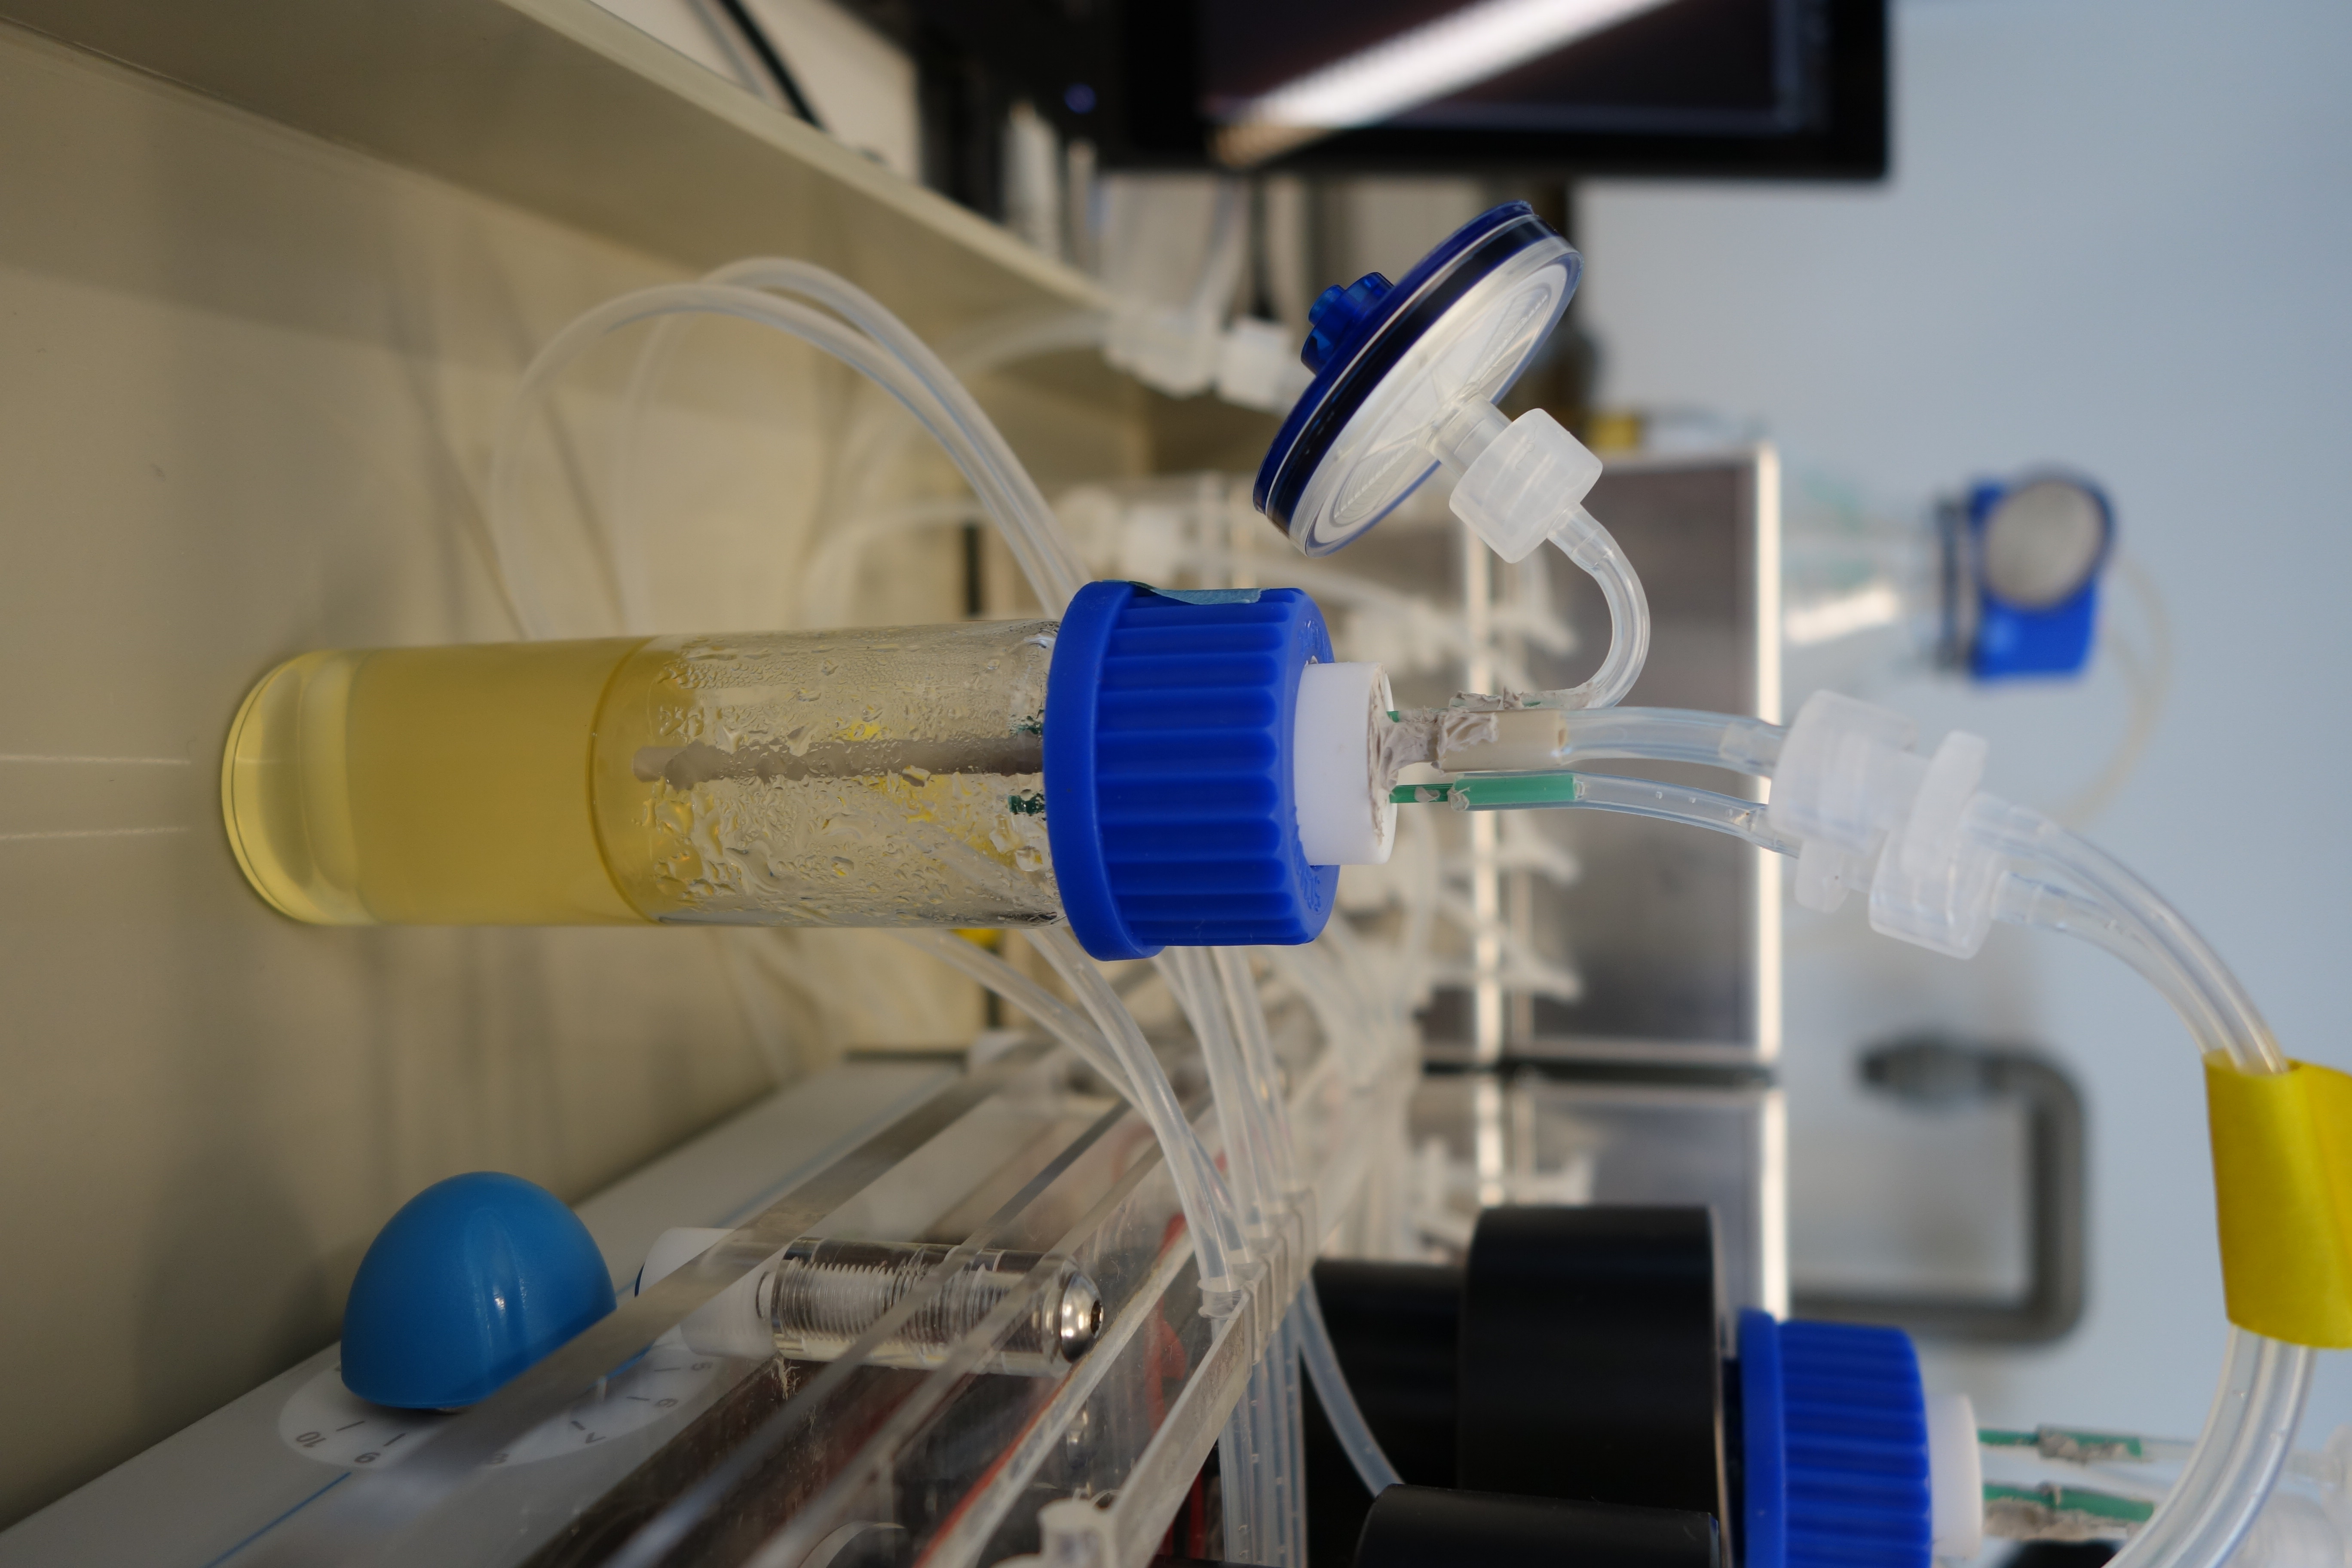
\includegraphics[angle=90,scale=0.15]{vial.JPG}
	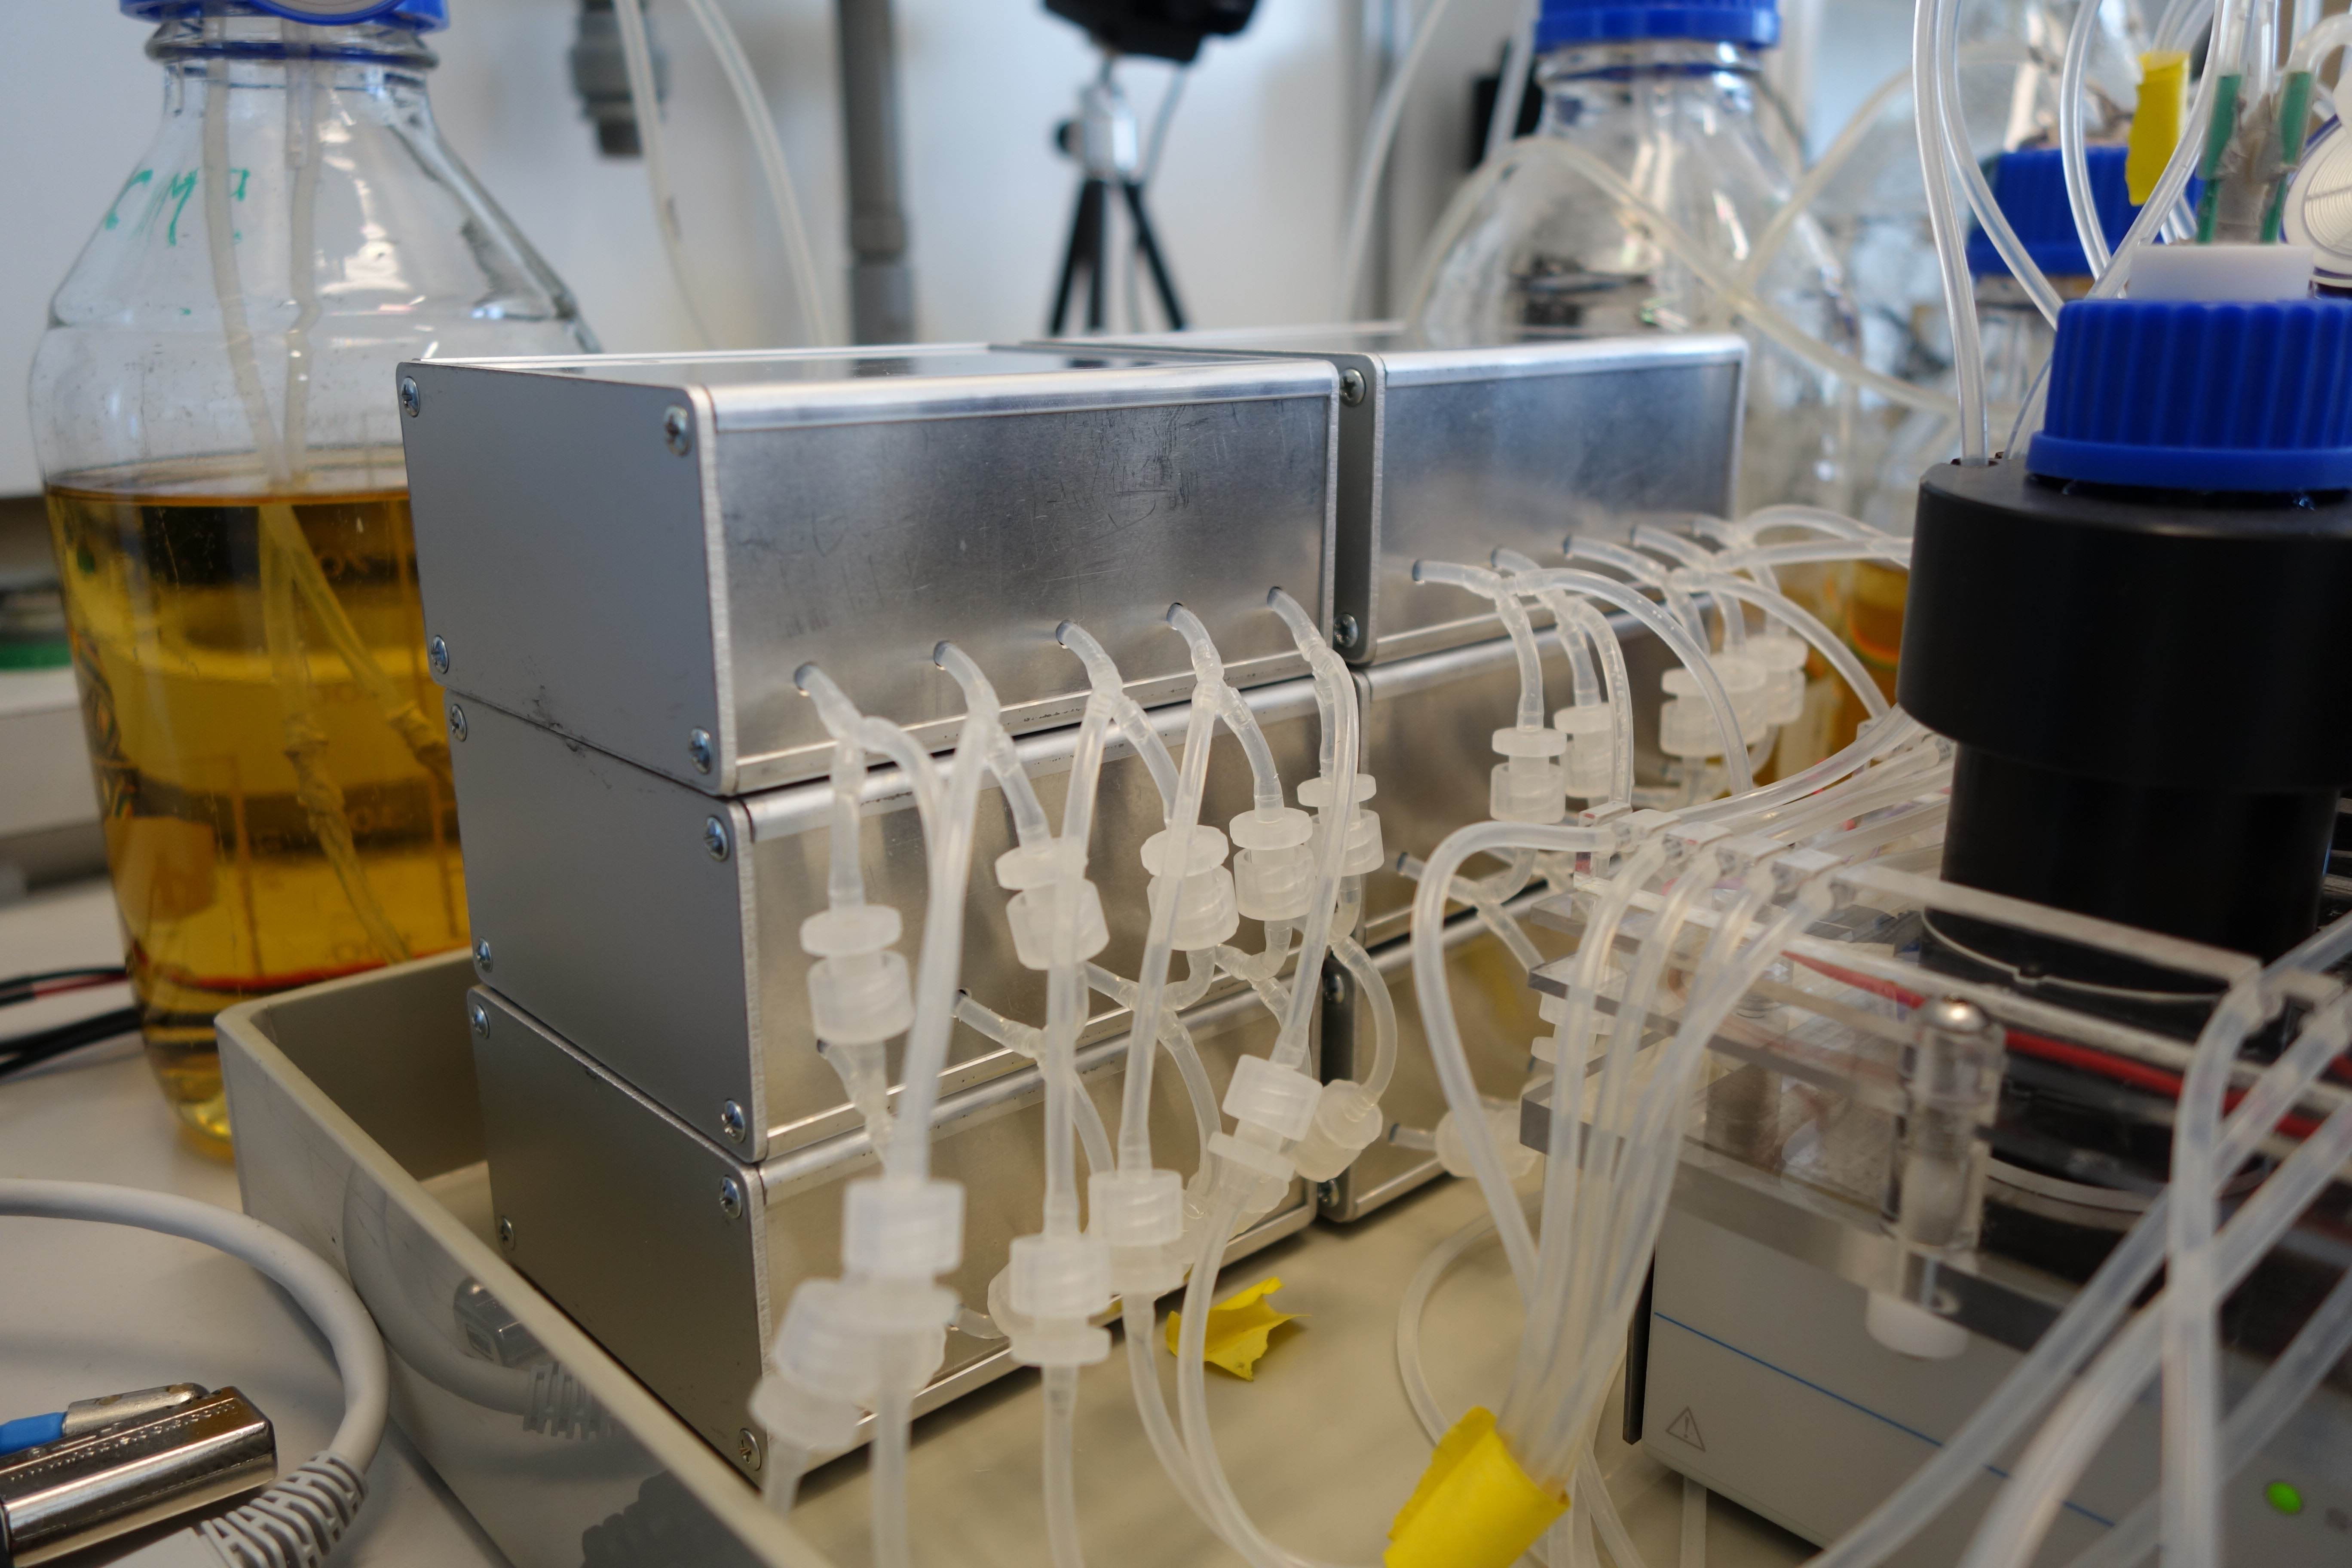
\includegraphics[scale=0.226]{pump_blocks.JPG}
	\caption{Figure left: Vial setup. Figure right: One row of five pumps represents one row of five vials. Since every vial is connected to three pumps, three rows of pumps are stacked on top of each other and connected column by column. This means that one column of three pumps is responsible for injection fluid into one vial. Every outlet from a pump from one column is connected, in order that there is just one tube going to one vial. }
	\label{figure:tubing_setup}
\end{figure}
Three connected injecting pumps per vial led to 45 injecting pumps in total. Mp6 pumps from microComponents were chosen because they have a compact built, having the size of half an USB stick. This is an improvement because the pumps used by Toprak et al \cite{toprak_building_2013} and Doesselmann \cite{doselmann_rapid_2017} were peristaltic pumps which were cubic with a size of approximately 4x4x4 cm. 

The functional principle is based on a piezoelectric diaphragm in combination with passive check valves which is shown in figure \ref{figure:piezo}. By applying voltage a piezo ceramic mounted on a membrane is deformed resulting in a down stroke. When the voltage decreases again the piezo deform again causing an upstroke of the membrane \cite{piezo_pumps}. Because the pump process depends on excitement and relaxation caused by the power, the flow rate generated by the pumps is dependent from the frequency. This also implements that the flow rate is very constant given that the power frequency is also constant. That being the case, the mixing of drug concentration was done by turning on the pumps for a calculated time.

In order to excite and relax the membrane and the piezopumps 230 Volts and a very steady power frequency were needed for this process, making it necessary to control every single pump with a specific mp6-OEM controller. This controller took an input power of 5 V and used about 30 mA of current. The Arduino was not capable of supplying this amount of current for every pump, therefor a separate power adapter was installed to supply the pumps. 

The pumps could be controlled by connecting one pin of the controller from the pump to a digital pin of the Arduino. 
If the pin from the controller was put to ground, the pumps were turned on, if the pin was connected to 5 V the pumps were off. Turning on/off the controller only worked well, when the change of power was very sudden. 
By adding a pull-down resistor between the digital pins and the ground from the Arduino we could avoid that there was always a very small current flowing through the digital pins. Furthermore it was decided to work with a serial connected inverter, implementing that when the digital pin was set to low, the inverter caused a power of 5 V which meant that the pumps were off. On the other hand when the digital pin was set to high, the inverter produced a power of 0 V which turned the pumps on.  
As a waste pump a 16-channel peristalitc pump was used which was directly controlled with a digital pin from the Arduino. 
\label{section:pumps}
\begin{figure}
	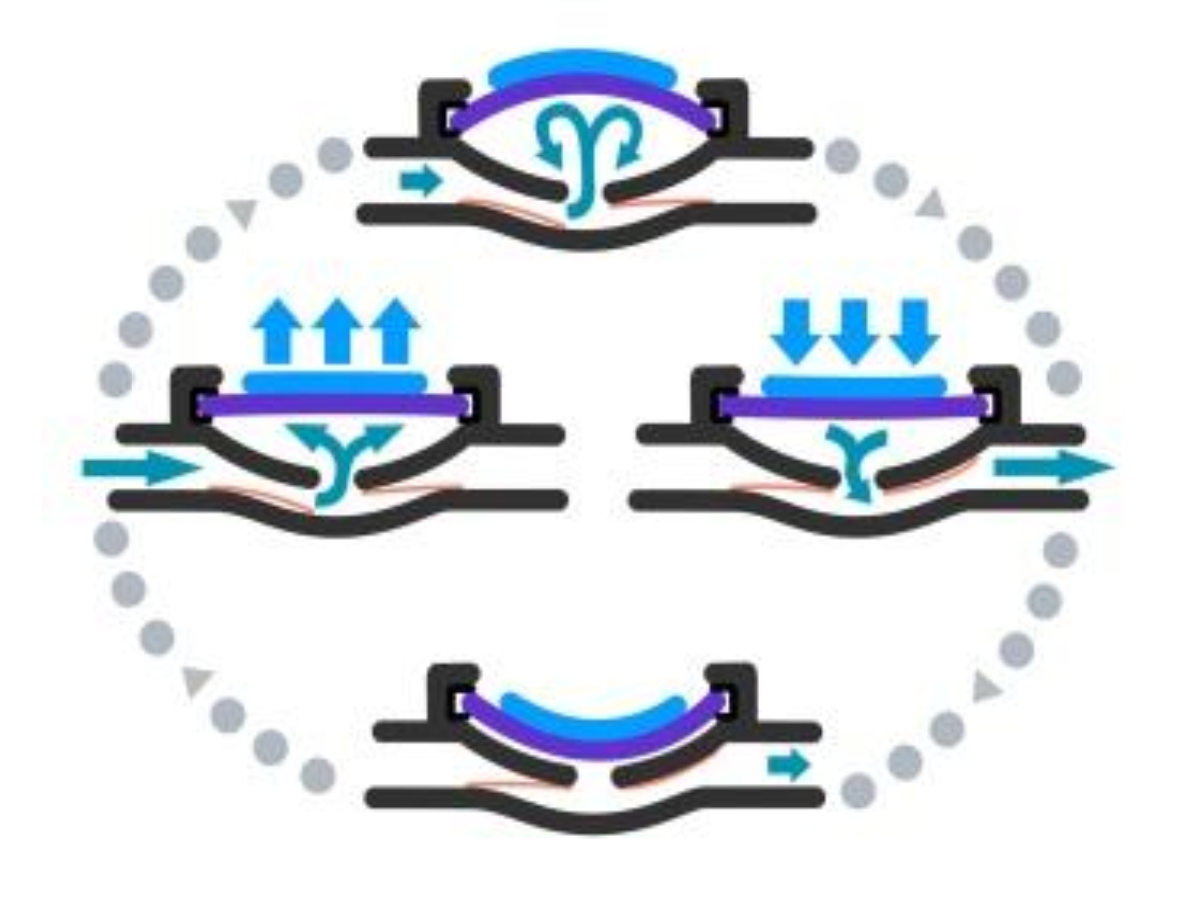
\includegraphics[scale=0.1]{piezo.png}
	%\includegraphics[]{circuit board}
	\caption{Principle of the mp6 pump but two of those piezoelectronics are connected in serial for this pump model \cite{piezo_pumps}}
	\label{figure:piezo}
\end{figure}

\subsection{Controlling of the morbidostat}
The controlling of the morbidostat was divided into two python scripts running on the laptop and one .ino script running on the arduino.
Communication of the two hardware devices was possbile via an USB cable enabling serial communication.
The two python scripts were arduino\_interface.py and morbidostat\_experiment.py. The arduino\_interface.py was responsible for transmitting commands to the arduino via the the serial connection but also for receiving data from the arduino. The arduino\_morbidostat.ino code interpreted the commands received from the laptop and excecuted hardware commands. Those commands were measuring voltages of analog pins, needed for the OD measuring, or truning on/off digital pins which turned the pumps on/off (see section \ref{section:pumps}).
The morbidostat\_experiment.py script on the other hand was responsible for saving data, initializing cycles and calculating appropriate drug concentrations. 
As shown in Figure \ref{figure:flowchart} the controlling of the morbidostat was done by constantly executing cycles. One cycle consisted of several steps depending on different scripts. \\
First the cycle itself was initiallized by morbidostat\_experiment.py and the ODs were measured and saved for every vial over the defined cycle time (typically 10 minutes). \\
Measuring of the OD as initialized by morbidostat\_experiment.py led to a function call in arduino\_interface.py which transmitted a command to the arduino. This command got interpreted and lead to measuring the voltages of the analog pins which were connected to an OD measuring unit as shwon in top right of the Figure \ref{figure:flowchart}. The resulting voltages got transmitted to the arduino\_interface.py via the serial communication. This script translated the voltages to optical densities according to a linear equation defined earlier by calibration. Morbidostat\_experiment.py was responsible for saving the ODs and averaging those values at the end of the cycle. As a next step a function in morbidostat\_experiment.py calculated how much drug should get added to which vial, based on the averaged ODs. The output of the function were runtimes of certain pumps. Those runtimes were transmitted again to the arduino via the arduino\_interace.py script and interpreted by the arduino. As shown in the last illustration of Figure \ref{figure:flowchart} the arduino switched the according digital pins to low for the time communicated from the laptop.
 
\begin{figure}
	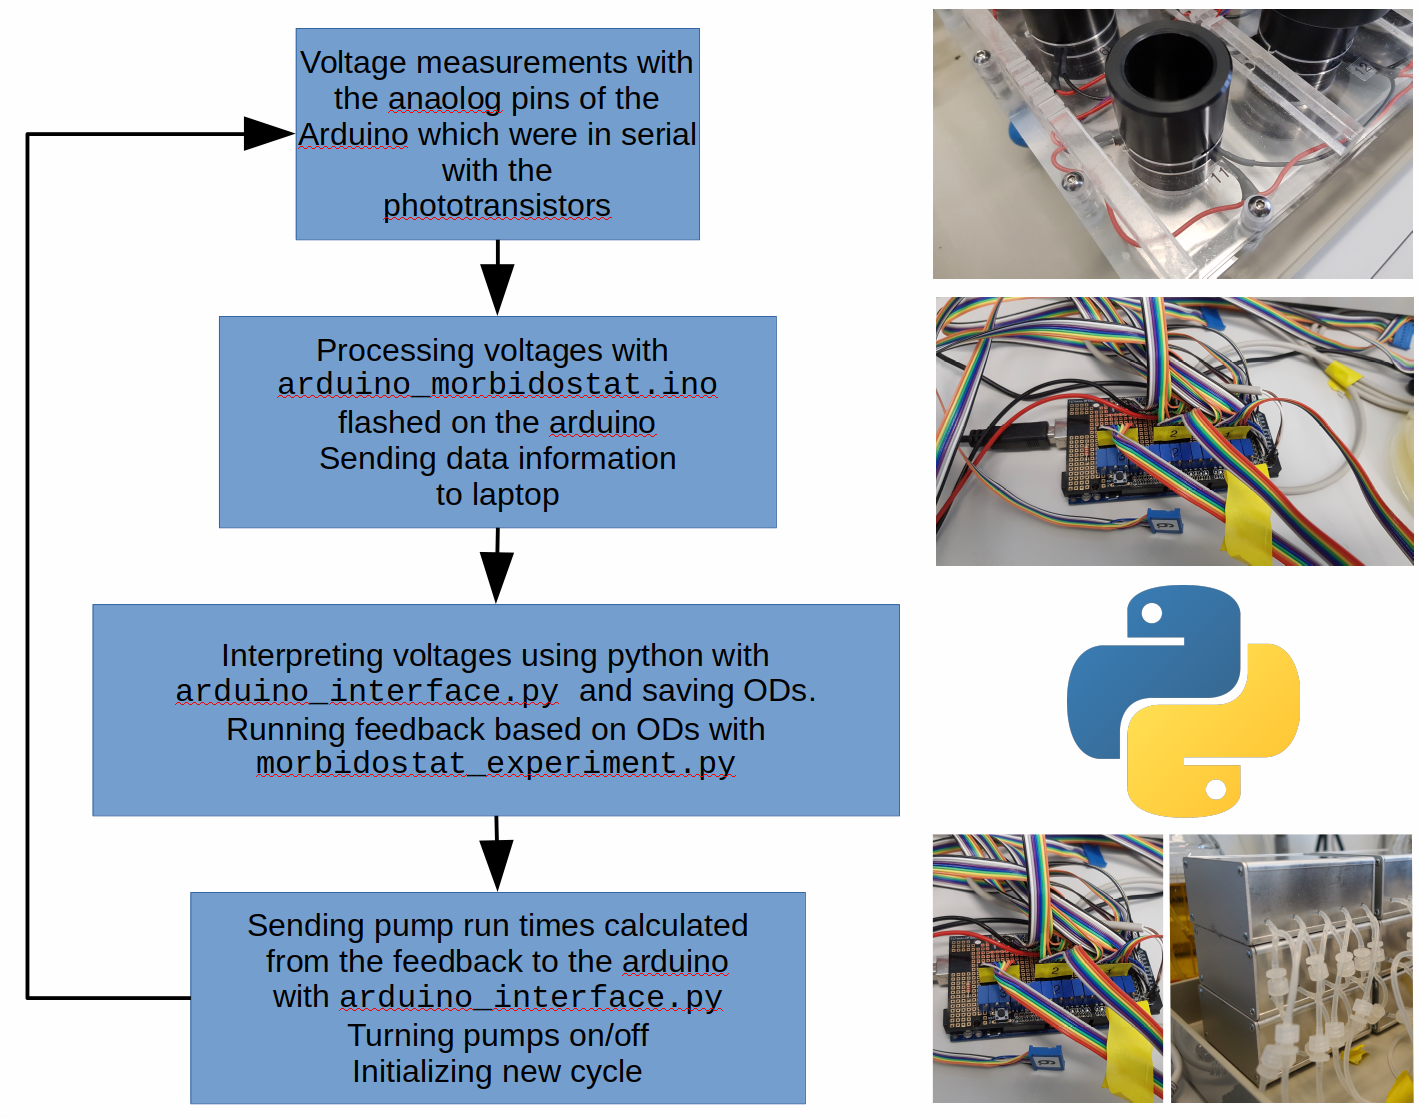
\includegraphics[scale=0.25]{flowchart.png}
	\caption{Overview of one cycle from the morbidostat.}
	\label{figure:flowchart}	
\end{figure}

\subsubsection{Feedback} 
The feedback coded as a function in morbidostat\_experiment.py was very important since it was responsible for putting the culture under antibiotic pressure. The outcome of the feedback depended on the growth of the bacteria. Therefor the growth was calculated at the end of every cycle bt calculating \textDelta OD according to the following formula:
\begin{center}
	$\Delta OD = (final\_OD[x_{cycles\_back}] - final\_OD[Cycle_{current})/x$
\end{center}
The final\_OD was calculated at the end of every cycle by averaging every OD measurment gathered over one cycle. As shown in the equation the difference between the final\_OD fromt the current cycle and the the final\_OD of x cycles back (x being typically 10) was calculated and divided by x.
As showin in Figure \ref{figure:feedback} the feedback did several comparisons before calculating an appropriate dose of drug. As a first step it checked if \textDelta OD was positive or negative. A negative \textDelta OD implied that the bacteria were dying. In order to prevent complete sterilization, media was getting added in this case. \\
When \textDelta OD was positive the bacteria were growing. Now it was important to not put the bacteria under selective pressure when the final\_OD of the cultures was were small (e.g. 0.03). If drug was added at this stage, this usually led to complete sterilization. That's why a threshold was introduced which was called drug\_dilution\_threshold. Therefor the next comparison as visible in Figure \ref{figure:feedback} was whether or not the final\_OD was higher or smaller than this threshold. If that was not the case the decision was nothing, which means that no fluid was added to the cultures. \\
However when the final\_OD was bigger than the threshold calculation of the appropriate dose was started.
This calculation depended on the MIC. Therefore the MIC had to be determined for the choesn bacteria and drug combination before the morbiostat experiment. Calculation of the concentration was divided into two equations consisting of an additive and a multiplicative component. The additive part was mainly important at the beginning of the experiment and was used to approximate a drug concentration in the vials similar to the MIC. Once the concentration in the vials was above the MIC the additive part was ignored. After that the current vial conentration was fed to an multiplicative equation. This equation multiplied the current drug concentration by the \textDelta OD which resulted in how much the drug concentration in the vial should be increased. This proved to be a good strategy, because fast growth meant stronger inhibition, but when the growth was very small and close to zero, the inhibition was not significantly increased. The multiplicative part also included other variables. For example a target\_OD was defined which was used to define which OD should not be exceeded. In general it was the goal to have the OD of the cultures close and steady to the target\_OD. \\
It was chosen to divide the outcome of the multiplicative component by this target\_OD. Therefor if the target\_OD was set to an high OD, inhibition was smaller than when set to a small OD. Furthermore variables had to be introduced to the multiplicative component which made it possible to make the feedback more aggressive or more sensitive.\\
Defining the target\_OD was a trade off of having a higher probability of mutations for a higher defined target\_OD, but keeping the culture at a high OD implemented fewer accuracy of the OD measurement caused by many dead cells.  


\begin{figure}
	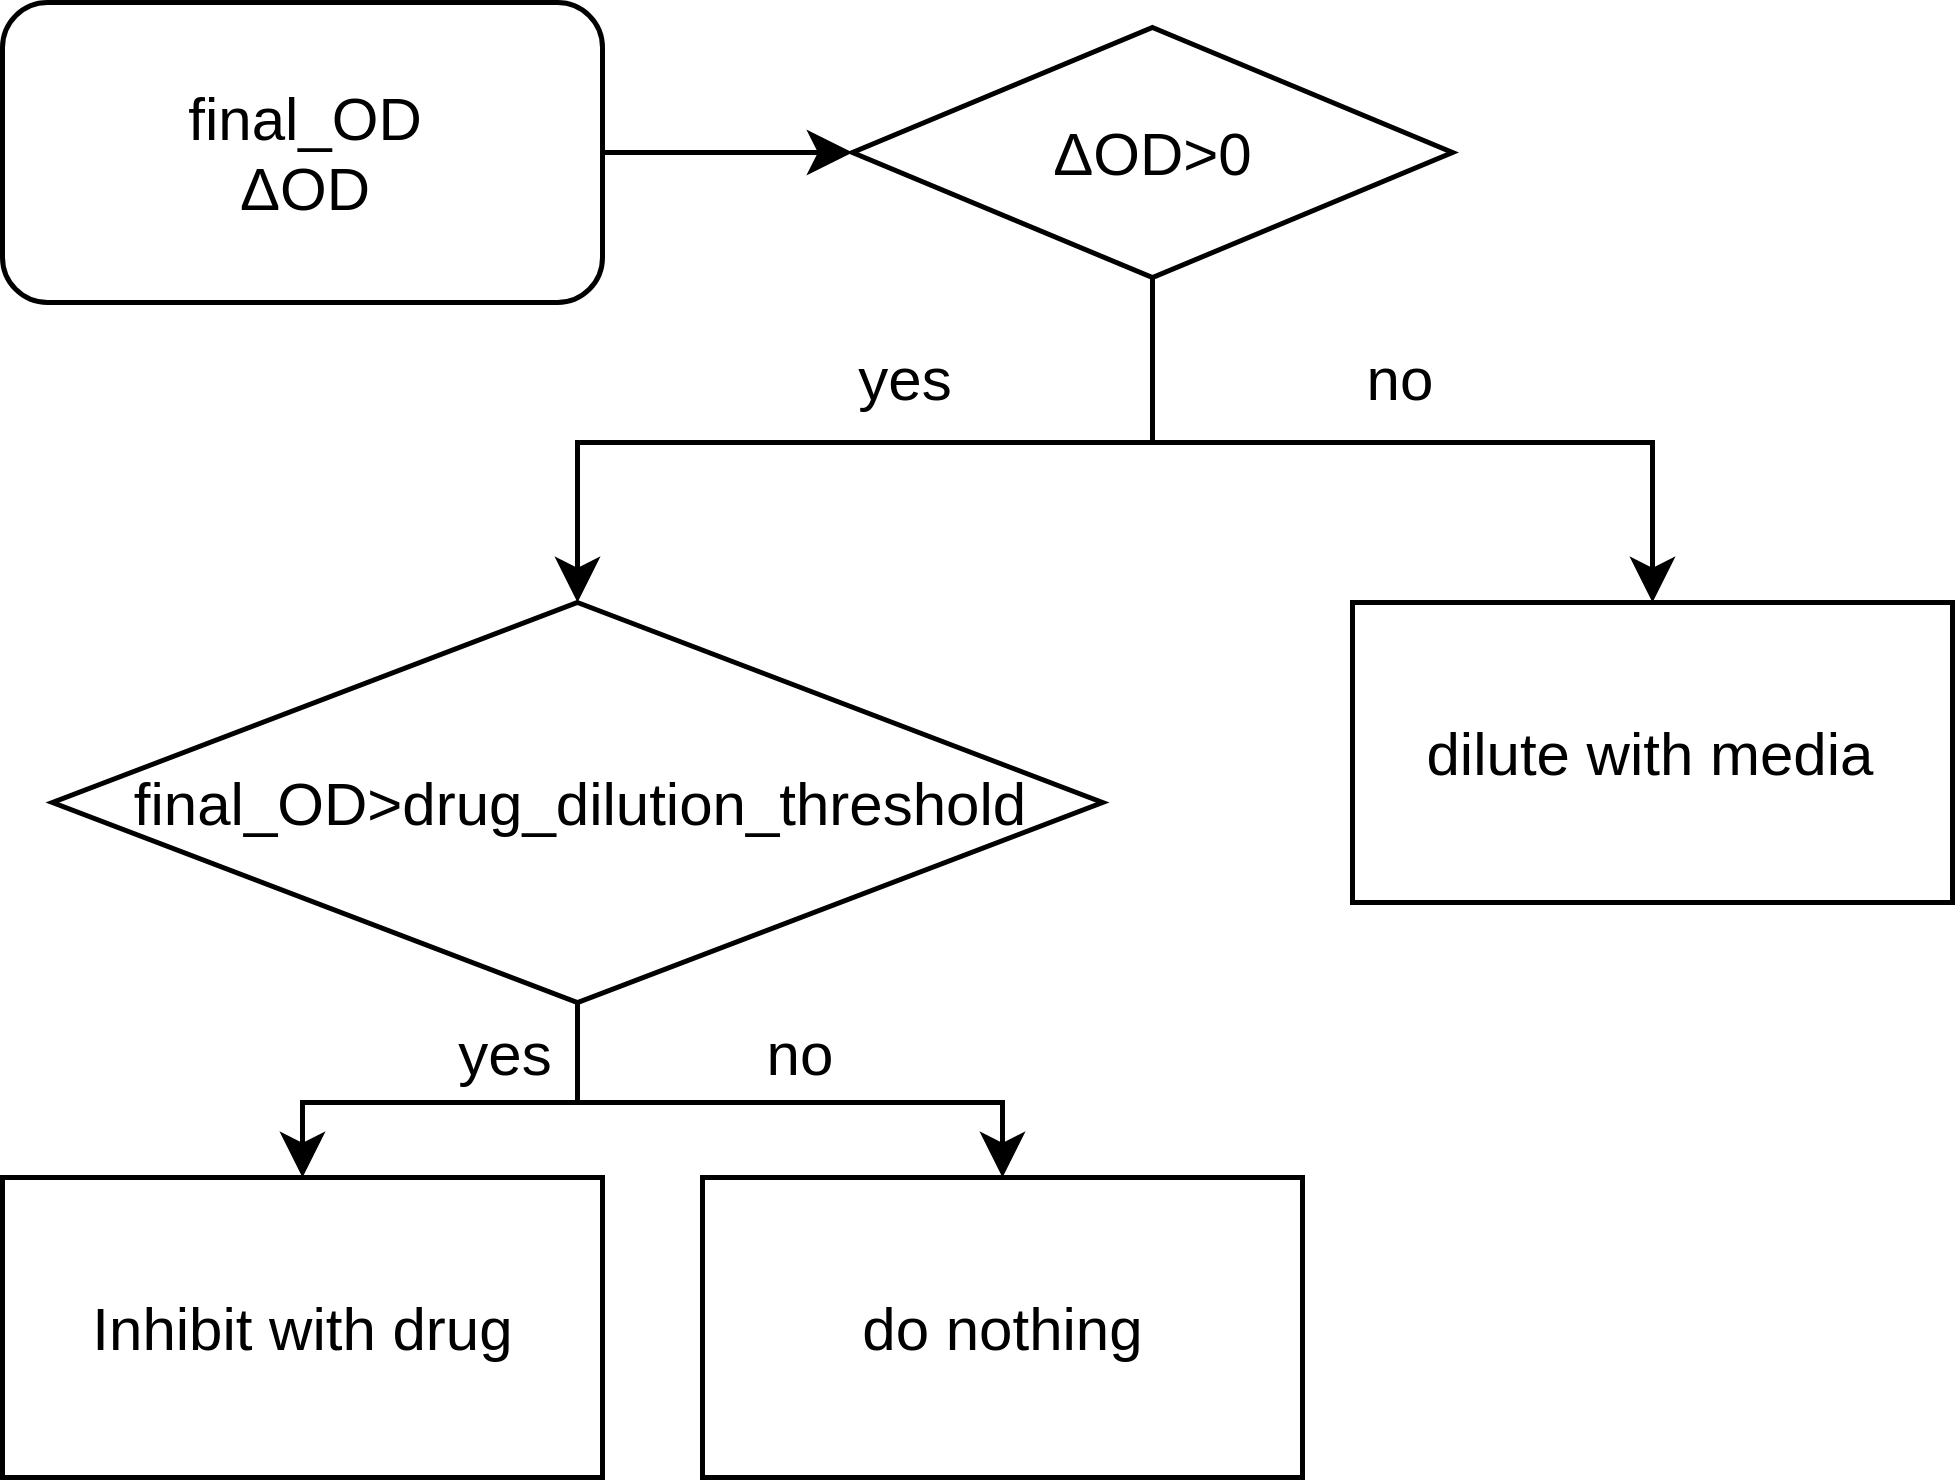
\includegraphics[scale=0.13]{feedback.png}
	\caption{Schematic overview of decisions involved in the feedback}
	\label{figure:feedback}
\end{figure}

\subsection{Experimental procedure}
\subsubsection{OD and pump calibration}
We chose 1/10 LB media and 9/10 $H_2O$ as a media for all experiments because the bacteria grew too fast by just using medi.. All the culturing of the bacteria was done in a 37 \degree \space incubator.  
For calibrating the OD measurements an overnight culure with K12 E. coli was inoculated in 5 ml diluted media. The next day the overnight culture was diluted 1/200 in 50 ml diluted media. After a few hours the OD of the culture was measured. Following ODs were prepared with 18 ml diluted media with the appropriate vials for the morbidostat: XXXXXXXXXXXXXXXXXXXXXXXXXXXXXX\\
Then every vial with of one certain OD was placed in every vial holder. With the function calibrate\_OD from the morbidostat\_experiment.py script, a current measurement was done for every OD and every vial holder. Because the current was measured for different ODs, the relation of current and OD could be described with a linear function. \\
For calibrating the pumps the function calibrate\_pumps from the morbidostat\_experiment.py was executed. This function demands the initial weight of every empty vial. After entering every weight, the function turned on every pump for 100 seconds. After that, the vials were weighted again and the values passed to the function which allowed precise calibration of each pump.
\label{section:OD_calibration}

\subsubsection{MIC determination}
Since the feedback was heavily dependent on the MIC, this value had to be determined for every drug which was used to run the morbidostat. Therefor 5 ml of MHB media was inoculated with the bacteria used for the actual experiment and cultured over night. The next day a 1/200 dilution in 20 ml MHB was prepared and cultured for a few hours. In the mean while a 128 fold concentration of the MIC found in the literature for the drug of interest was prepared in MHB. 128 fold was chosen, because the determination was done in a 96 well plate which implements that the MIC found in the literature is in the middle of the plate. The growth of the diluted culture was constantly monitored by measuring the OD. When the OD of the diluted culture was at 0.08, a 1/100 dilution was done once again. From this final dilution 100 \textmu l was pipetted in every well from the 96 well expect in the wells from the last column of the plate. Additionally 100 \textmu l of MHB was added to every well. As a next step 100 \textmu l from the prepared drug solution was added to the first column of the plate. Then 100 \textmu l from this column was transferred to next column and mixed. This was repeated until the third last column. This implements that the second last column acts as a control of the cells, since no drug was added. The last column acts as a control for the media. After preparing the well plate it was incubated for 16 hours at 37 \degree \space and after that, the OD of every well was measured using a plate reader. As MIC the columnof a certain concentration which inhibited the culture significantly was chosen.
\label{section:mic_determination}


\subsubsection{Sterilization of the morbidostat}   
In order to prevent contamination a solution with sterile water containing 3 \% bleach was prepared and pumped through every pump for 5 minutes. After that we let the solution sit in the tubes for about an hour. Afer that every tube was flushed with sterile water by pumping it through every pump for 5 minutes. All the media, drug bottles and vials with its luer connections were autoclaved before the experiment.
\label{section:sterilization}

\subsubsection{Testing the continuous culture mode from the morbidostat}
An overnight culture was set up by inoculating 5 ml of diluted media with K12 XL1-Blue E. coli. The next day a 1/200 dilution in 200 ml was prepared and 18 ml of this suspension was pipetted in 18 sterile vials. A grow curve was determined by starting an experiment with the morbidostat in the GROWTH\_RATE\_EXPERIMENT modus. The morbidostat was put in the hypoxi-station at 37 \degree \space with an air composition of \_ \% $CO_2$ and \_ \% nitrogen. The growth rate experiment was done overnight. The next day ideal dilution rates for the continuous experiment were identified, by feeding the growth rates to the \href{https://github.com/nahanoo/ESBL\_project/}{morbidostat\_simulator.py} script which simulates a continuous morbidostat experiment. Also the best parameters for te feedback were determined using the simulator.
As a drug amoxicillin was chosen, it's MIC was determined as 2 \textmu/ml according to the procedure in \ref{section:mic_determination}. As a starting concentration 6 \textmu/ml and 14 \textmu/ml 
were chosen for the drug bottles. Tubing, bottles and vials were sterilized according to the section \ref{section:sterilization}. The continuous morbidostat experiment was started by initializing the experiment with the 	CONTINUOUS\_MORBIDOSTAT modus under the same temperature and air condition as for the grow curve determination. The dilution\_factor was set to 0.94. Every other day 200 \textmu of the suspension in the vials were transferred into new sterile vials filled with 18 ml diluted media. When a drug bottle was empty, the MIC was changed in the morbidostat\_experiment.py according to the concentration which was needed to strongly inhibit the growth. New drug concentrations were chosen based on the newly determined MIC. For the lower concentrated bottle a 3 fold MIC concentration, was chosen. For the higher concentrated drug bottle the concentration was set to 7 fold MIC. At day 4 of the experiment, samples were taken from every vial, by opening the vial in the hypoxi-station and transferring 200 \textmu into eppendorf tubes. Those samples were cultured over night in 5 ml diluted media and the next day the MIC was determined. The morbidostat experiment was stopped after 6 days.

\section{Plasmid construction}
\subsubsection{Primer design}
In total x plasmids were produced with the gibbson assembly cloning procedure. For every \textbeta-lactamase found in every sample of interest a plasmid was produced. As target sequences every \textbeta-lactamase sequence with it's upstream sequence until the previously located gene plus 50 additional base-pairs was chosen. 





 